\documentclass[../main.tex]{subfiles}

\begin{document}

\chapter{Introduction}
\label{chap:introduction}
For this thesis, the key question we are attempting to ask is this:
\medskip 

\begin{tcolorbox}[colback=white!98!black,colframe=gray!60!blue]
\centering
	\textit{What drives the trends and variability we see in Antarctic ice?}
\end{tcolorbox}

Our motivation for asking this is as follows. Ice in Antarctica is critical for our understanding of global climate patterns and climate change. It has a high albedo and stores massive amounts of both energy and water, being intrinsically linked with both the water cycle and energy balance for the Southern Hemisphere. Sea ice melts and reforms around the continent each year, trapping extra C0$_2$ in the Ocean. It is also shown to affect the salinity of the ocean and ocean circulations. 
The extent of ice is additionally linked to the state of the climate in Antarctica, and therefore by extension, the state of our global climate. Understanding the processes which have driven its behaviours and which could potentially drive the trends and variability we see in both land and sea ice in Antarctica in the future is therefore important for our understanding of the changing climate of Earth.

In order to answer our question we will make use of statistical techniques such as linear regressions and Pearson correlations to determine the relationships which we can observe between ice in Antarctica, different environmental variables such as temperature, Ozone concentration, and surface pressure, and climatic patterns which are known to drive global and southern hemisphere climate such as the El Ni\~no Southern Oscillation and the Southern Annular Mode.

This introduction will include details about the data we have used in this project, followed by a brief overview of the analysis carried out on the data and a discussion of our key findings. The rest of the thesis will cover the analysis and results in more detail alongside a literature review which should introduce the key ideas which you need to know to understand the state of contemporary research on ice in Antarctica and its relationship with global climate.


\section{Data used in this project}

For this project we used a wide variety of data sources, detailed in more detail in the Data chapter of this thesis. We will briefly comment on what sources were used for each dataset and variable here.

For sea ice, we used concentration from Nimbus-7 SMMR and DMSP SSM/I-SSMIS Passive microwave data, provided by NSIDC. For the thickness of sea ice we use data from \todo{where?}. For land ice thickness and volume, we sourced data from the NASA GRACE mission. 

Additionally to the variety of sources for Antarctic ice, we also used data for a number of ``environmental variables'' such as temperature and ozone concentration. These are almost entirely sourced from the ECMWF ERA5 reanalysis. Temperature values are verified against station data around Antarctica to ensure that it is of high quality. (See the Data chapter of this thesis for more detail.)

\section{Planning the analysis}
\todo{This can be like Figure \ref{fig:flowchart} or the next section of this introduction. Finish this at end of project when we know what we did.}
\begin{figure}[hbt!]
    \centering
    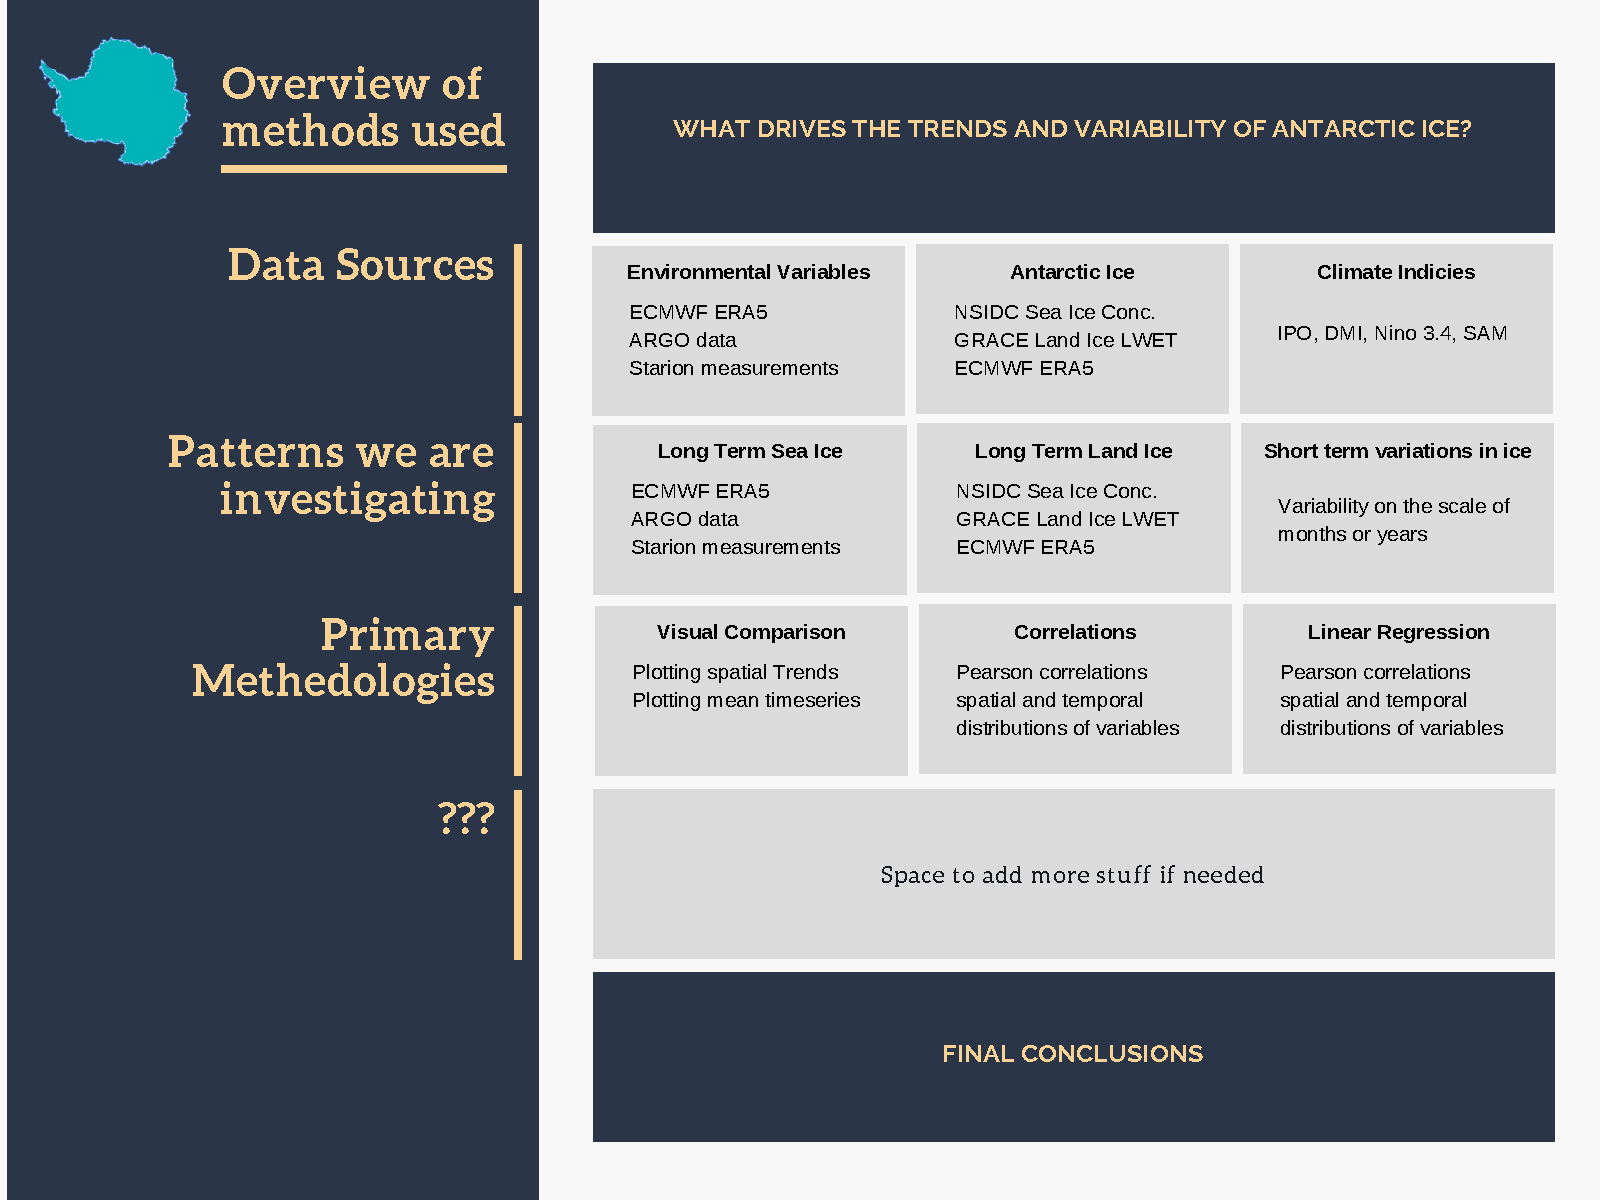
\includegraphics[width=\textwidth]{images/flowchart/Flowchart of analysis and methods.pdf}
    \caption{Option one}
    \label{fig:flowchart}
\end{figure}

\section{Structure of the methods used}
Below we will go into more detail about how each of the procedures mentioned here work and are implemented, however first, let's take a moment to outline the processes carried out on the data for our analysis.
\begin{enumerate}
    \item \textbf{Data Wrangling}. First we had to manipulate the raw data for analysis. 
    \begin{enumerate}
        \item \textbf{Standardise the data}. The data came from a variety of sources. The idea here is that regardless of the source, we can process everything in the same manner.
        \item \textbf{Change the resolution}. By lowering the resolution of the data we can speed up our computation. Higher resolutions return better quality results. We did this both temporally and spatially.
        \item \textbf{Regridding}. In some of the computations, we required the data to represent set coordinates.
        \item \textbf{Temporal decomposition}. We performed analysis for both standard time series and anomalous time series for each set of data.
        \item \todo{[WIP]} \textbf{Smoothing of data}. In order to make the analysis easier to analyse, we applied band-pass filters and moving averages to a variety of time series. 
    \end{enumerate}
    \item \textbf{Correlation analysis}. Our first analysis technique revolved around Pearson correlation coefficients between different time series. 
    \begin{enumerate}
        \item \textbf{Correlations}. The primary output here is the correlation between the different time series we are analysing.
        \item \textbf{P-values}. In order to identify how significant our results are we used p-values from a Student's t-test \todo{(confirm this)}.
        \item \textbf{Compare time series}. As a visual check for the validity of results, we also plotted example time series of the different correlated variables used.
        \item \todo{[WIP]} \textbf{Time-lagged correlations}.
    \end{enumerate}
    \item \todo{[WIP]} \textbf{Regressions}. In order to quantify the impact different variables have on each other we turned to a multivariate regression analysis.
    \item \todo{[WIP]} \textbf{Temporal breakdown}. In order to identify specific patterns in the data we broke the temporal scale up in a number of ways.
    \begin{enumerate}
        \item \todo{[WIP]} \textbf{Extreme events}. By taking times when the SIE was at extreme values, we can look at patterns seen in different variables and indices and link what is observed to physical processes.
    \end{enumerate}
\end{enumerate}



\section{Our key findings}
Our final point of importance before launching into the main body of this thesis is a quick summary of our key findings.
\begin{itemize}
    \item Temperature statistically accounts for the majority of trends and variability in Antarctic Sea Ice.
    \item Local temperature does not statistically account for the trends and variability in Antarctic Land Ice, however remote temperatures seem more promising.
\end{itemize}

\end{document}